\section{Results}
\label{sec:results}

Errors are relative $L^2$ against the reference solution, as the median over five seeds.
Table~\ref{tab:claims} lists every pre-registered claim about the one-copy circuit and
Table~\ref{tab:ensemble} those about the eight-copy circuit; the sections below take the
evidence question by question.

% Generated by scripts/report/paper_tables.py from results/adjudication_v1_full.json.
\begin{table}[htbp]
  \centering
  \small
  \begin{tabular}{p{0.5\linewidth}lr}
  \toprule
  Claim & Verdict & Measured \\
  \midrule
  Beats the large MLP on Poisson ($\ge2\times$) & Refuted & 0.65$\times$ \\
  Beats Fourier features on Poisson ($\ge1.3\times$) & Refuted & 0.13$\times$ \\
  Matches the frequency-matched classical model on Poisson (within $1.3\times$) & Refuted & 5.11$\times$ \\
  Heat: no model beats the MLP by more than 5\% & \textbf{Confirmed} &  \\
  Helmholtz: the gain over the MLP grows with $k$ & \textbf{Confirmed} &  \\
  Designed beats random frequencies, Poisson ($\ge1.5\times$) & Inconclusive & 1.84$\times$ \\
  Designed beats random frequencies, heat ($\ge1.5\times$) & \textbf{Confirmed} & 6.52$\times$ \\
  NTK flatter inside $\Omega$ than outside, Poisson & Insufficient data &  \\
  NTK flatter inside $\Omega$ than outside, Helmholtz $k{=}10$ & Refuted & gap -8.4 \\
  Gain over the MLP lies inside $\Omega$, Poisson ($\ge70\%$) & \textbf{Confirmed} & 99.9\% \\
  Gain over the MLP lies inside $\Omega$, Helmholtz $k{=}10$ & Refuted &  \\
  Higher coverage gives lower error ($\rho\le-0.7$) & Refuted &  \\
  Gradient variance stays above the barren-plateau line & \textbf{Confirmed} & slope 0.31, $R^2$ 0.001 \\
  Leaves the lazy-training regime earlier than classical models & Refuted & 1.01 vs 4.3e+06 \\
  Encoder drift stays below 0.2, so $\Omega$ stays valid & \textbf{Confirmed} & 0.13 \\
  \midrule
  Confirmed & 6 of 15 & \\
  \bottomrule
  \end{tabular}
  \caption{Pre-registered claims about the one-copy SMCD circuit, seeds 0--4, as the adjudication
    script scores them. Ratios are baseline error over circuit error, except the
    frequency-matched comparison (circuit over baseline) and drift (hybrid vs classical).}
  \label{tab:claims}
\end{table}


\subsection{The circuit realises its design}
\label{sec:realise}
For every one-dimensional problem, the SMCD circuit was evaluated at 40 random parameter
settings and its output Fourier-transformed. The largest amplitude outside the designed
set $\Omega$, relative to the largest overall, is at most $3.8\times10^{-15}$, i.e.\
floating-point zero (Figure~\ref{fig:circuitspec}), and the test suite checks the same
property on every build. The encoder that feeds the circuit could in
principle move $\Omega$ during training, but it barely does: the drift $\|A-I\|_F$ at the
end of training is 0.13 for one copy and 0.10 for eight, under the 0.2 at which the
coverage computed at initialisation would stop describing the trained model. The design
card is therefore a statement about the trained model, not only its starting point.

\begin{figure}[htbp]
  \centering
  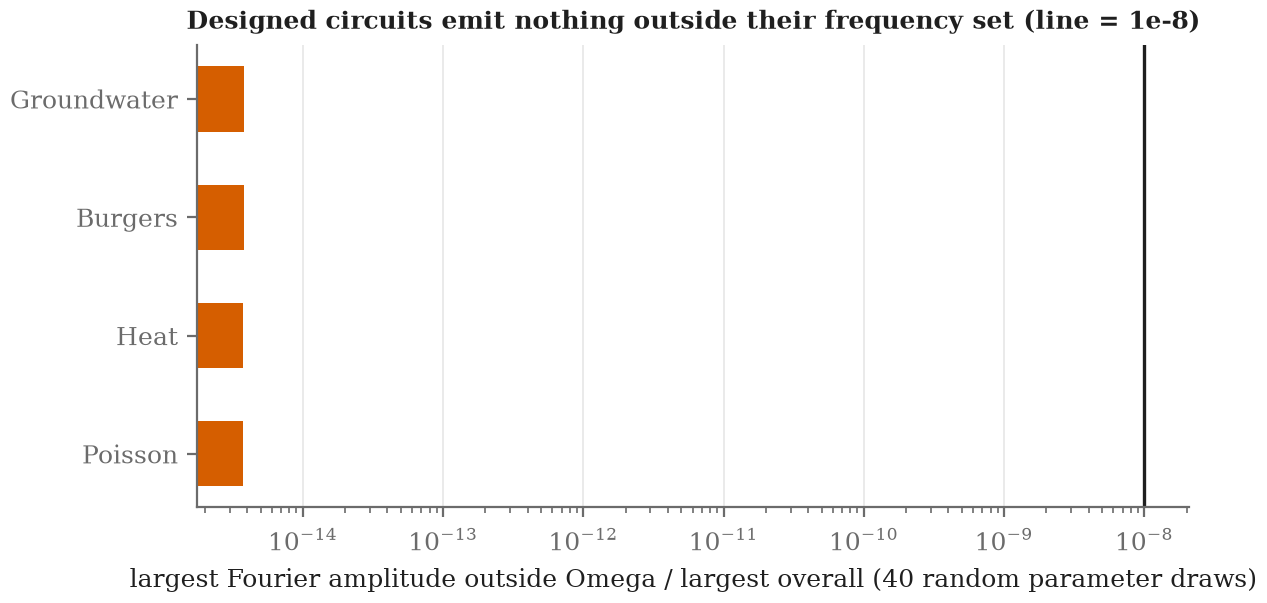
\includegraphics[width=0.5\linewidth]{../results/report/figures/validation_circuit_spectrum.png}
  \caption{Largest Fourier amplitude outside $\Omega$ for each problem's SMCD circuit,
    over 40 random parameter draws (line: $10^{-8}$). The two-dimensional Helmholtz
    designs are not covered by this one-dimensional check.}
  \label{fig:circuitspec}
\end{figure}

\subsection{Accuracy across six problems}
\label{sec:accuracy}
Table~\ref{tab:accuracy} and Figure~\ref{fig:accuracy} give every family's error on every
problem with one copy of the circuit. Three regimes appear.

\begin{table}[htbp]
  \centering
  \footnotesize
  \setlength{\tabcolsep}{4pt}
  \begin{tabular}{lrrrrrr}
  \toprule
  & & & & \multicolumn{3}{c}{Helmholtz} \\
  Family & Poisson & Heat & Burgers & $k{=}4$ & $k{=}10$ & $k{=}20$ \\
  \midrule
  MLP & 1.08 & \textbf{0.305} & \textbf{0.014} & $\mathbf{5.0\times10^{-5}}$ & 1.00 & 1.00 \\
  Fourier features & \textbf{0.21} & 0.39 & 0.33 & 0.92 & 1.00 & 1.00 \\
  Frequency-matched & 0.33 & 0.33 & 0.31 & 0.95 & 1.00 & 1.00 \\
  SMCD circuit & 1.68 & 0.42 & 1.14 & 1.59 & 1.09 & 1.00 \\
  Random frequencies & 3.08 & 2.74 & 1.06 & 0.95 & 1.01 & 1.01 \\
  Parallel hybrid & 0.35 & 0.76 & 0.26 & 0.26 & 1.00 & 1.00 \\
  Octave ensemble & 0.75 & 0.68 & 0.85 & 1.00 & 1.00 & 1.00 \\
  \bottomrule
  \end{tabular}
  \caption{Median relative $L^2$ error, one copy of each circuit, seeds 0--4 (two to four
    seeds for six Helmholtz $k{=}10$/$20$ cells). Bold: best per problem. Predicting
    $u\equiv0$ scores exactly 1.}
  \label{tab:accuracy}
\end{table}

\begin{figure}[htbp]
  \centering
  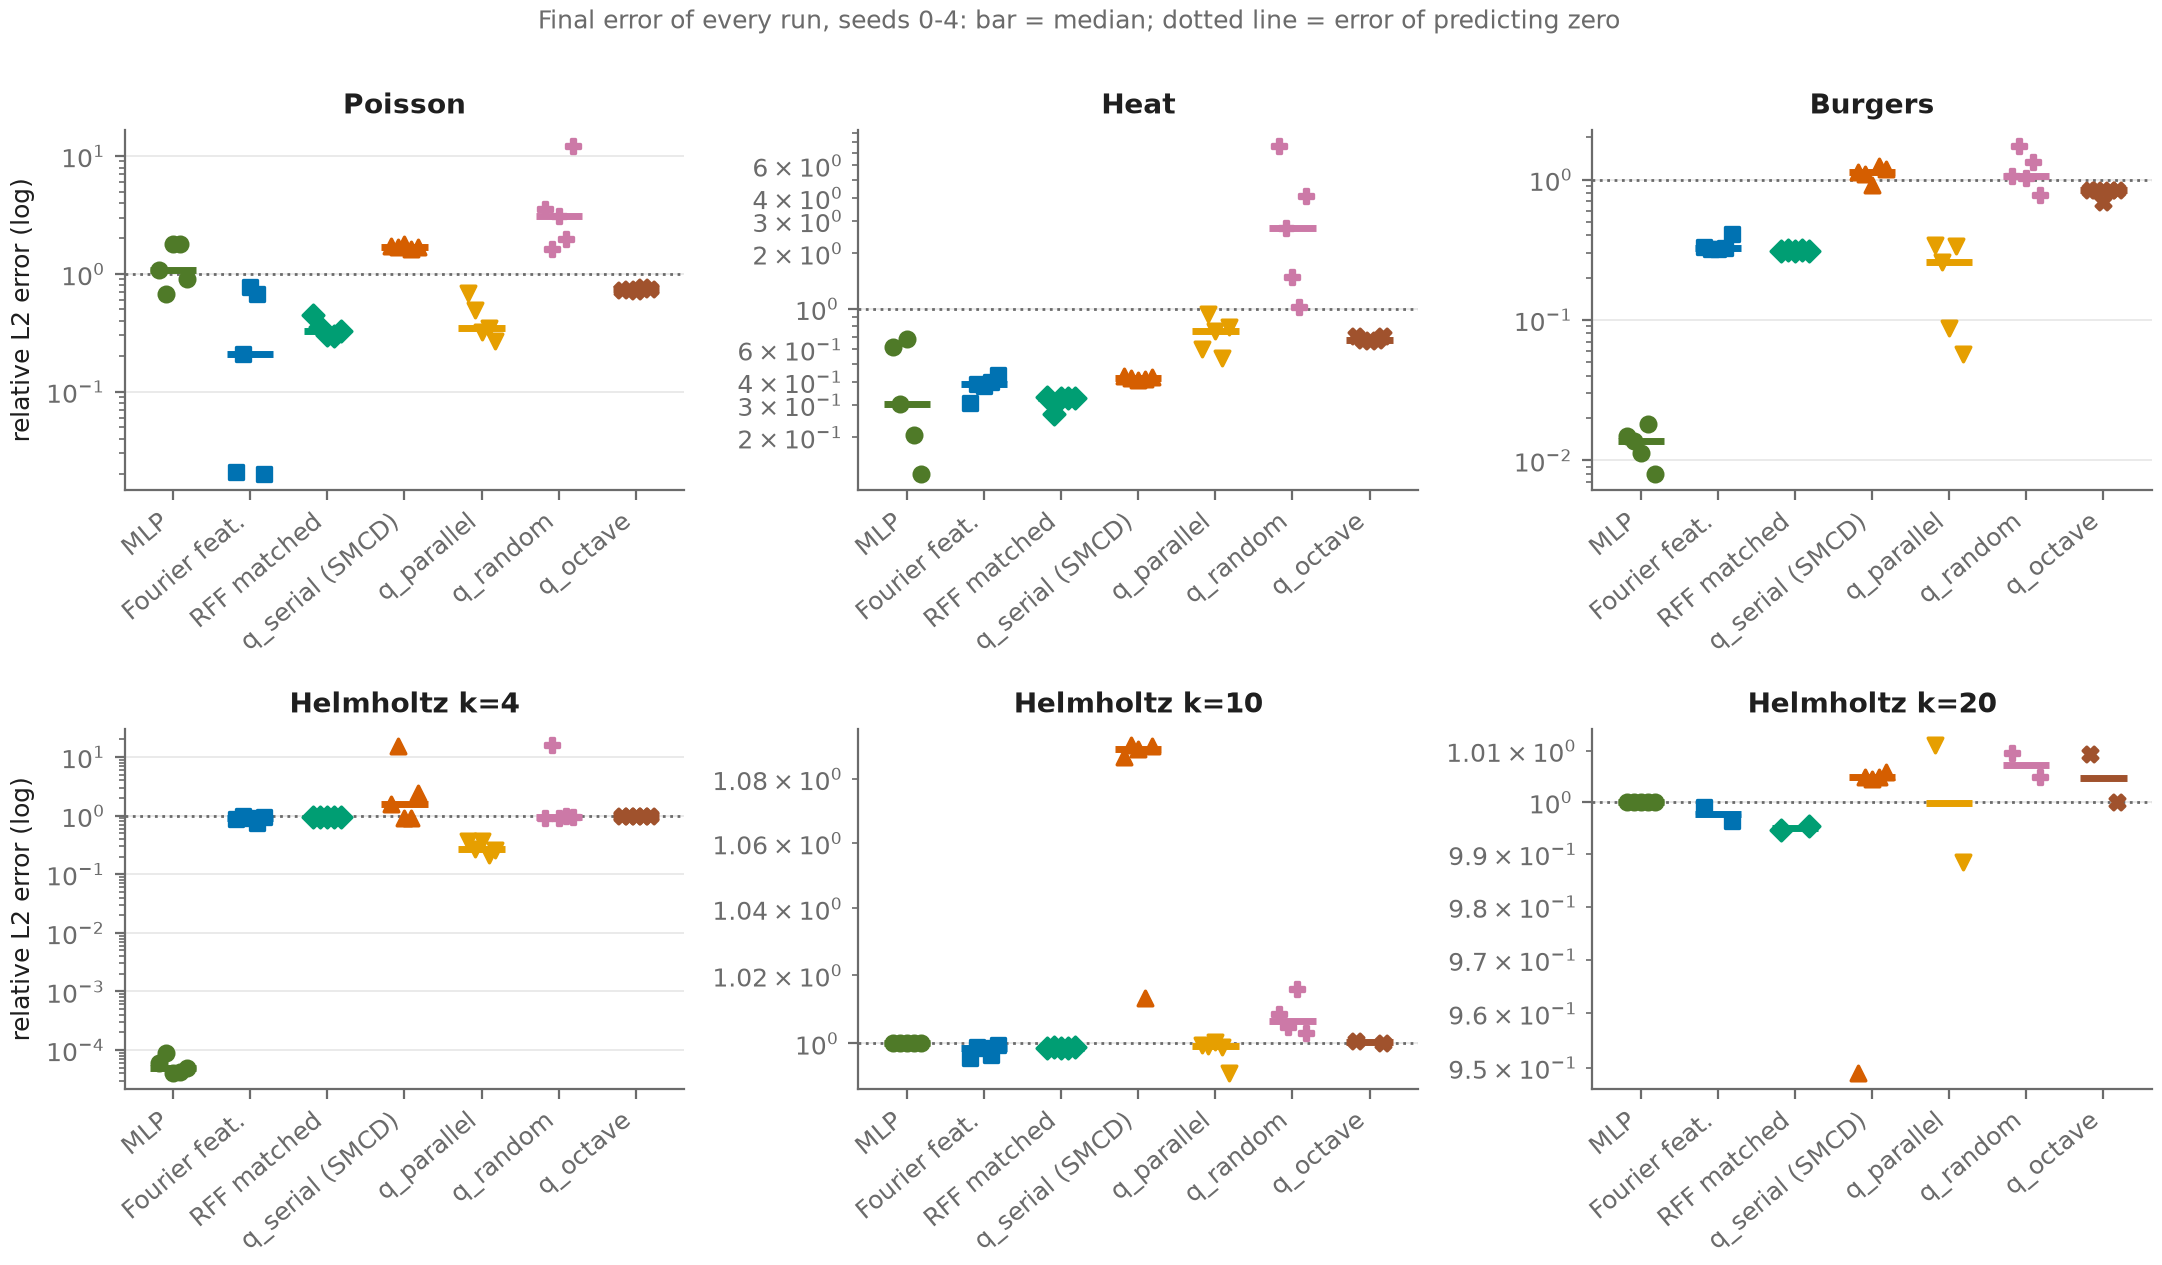
\includegraphics[width=\linewidth]{../results/report/figures/accuracy_all_runs.png}
  \caption{Final relative $L^2$ error of every run, per problem and family.}
  \label{fig:accuracy}
\end{figure}

\paragraph{Where a slow and a fast wave mix (Poisson, Burgers, Helmholtz $k{=}4$),
classical models win against one copy.} On Poisson the circuit's error (1.68) is higher
than the MLP's (1.08), the Fourier-feature network's (0.21) and the frequency-matched
model's (0.33); all three comparisons are refuted. Section~\ref{sec:copyresult} traces
this to coupled amplitudes and removes it with copies.

\paragraph{On a smoothing operator (heat), nothing beats a plain MLP.} SMCD predicts
this before training (Proposition~2): diffusion removes the high-frequency content a
circuit could supply, and the design card's predicted benefit is 2.5\%. Every family is
worse than the MLP, the circuit by 38\% and the random-frequency circuit by $9\times$, so
the claim that no family beats it by more than 5\% is confirmed.

\paragraph{At high wavenumber (Helmholtz $k{=}10,20$), every model fails.} Every
family's median error is 0.995--1.09, the score of predicting zero. The pre-registered
trend that the circuit's error ratio against the MLP improves with $k$ is confirmed
($3\times10^{-5}\to0.92\to0.99$), and the circuit is within $1.3\times$ of the
frequency-matched model at both wavenumbers, but both are parity among models that did
not learn the solution. A plausible cause, not tested here: at these $k$ the forcing
term is about 1\% of the Laplacian term, so $u\equiv0$ leaves a small residual. SMCD's
own predicted benefit is zero at $k=4$ and $k=10$.

\paragraph{Cost.} On a classical simulator a circuit run takes a median of about
2{,}900\,s, against 330--590\,s for the classical families, with the same number of
optimiser steps.

\subsection{Designed frequencies beat random ones}
\label{sec:design}
The sharpest test of SMCD holds the circuit, its size and its training fixed and changes
only the encoding scalings, from SMCD's to random ones (Figure~\ref{fig:designrandom}).
Random scalings drawn from $U(0.5,3)$ reach at most about 12 radians per unit in four
layers, short of the $15\pi\approx47$ wave, so the comparison tests whether reaching the
needed band matters. Wherever the circuit learns the solution, it does:

\begin{itemize}
  \item \textbf{Heat, one copy:} $6.5\times$ lower error on all five seeds (95\%
    bootstrap interval 2.5--17.7$\times$, Section~\ref{sec:validation}). The designed
    circuit is also the most consistent model in the matrix (worst over best seed within
    4\%), while its random twin is the least ($7.4\times$).
  \item \textbf{Poisson, eight copies:} $236\times$ (0.0037 against 0.87), all five
    held-out seeds.
  \item \textbf{Groundwater, eight copies:} $9.9\times$ (0.09\% against 0.92\%), all five
    held-out seeds (Section~\ref{sec:groundwater}).
\end{itemize}
On Poisson with one copy the median ratio is $1.84\times$, but one seed of five
disagrees, so the claim is inconclusive; this is the case where one copy does not learn
the solution at all.

\begin{figure}[htbp]
  \centering
  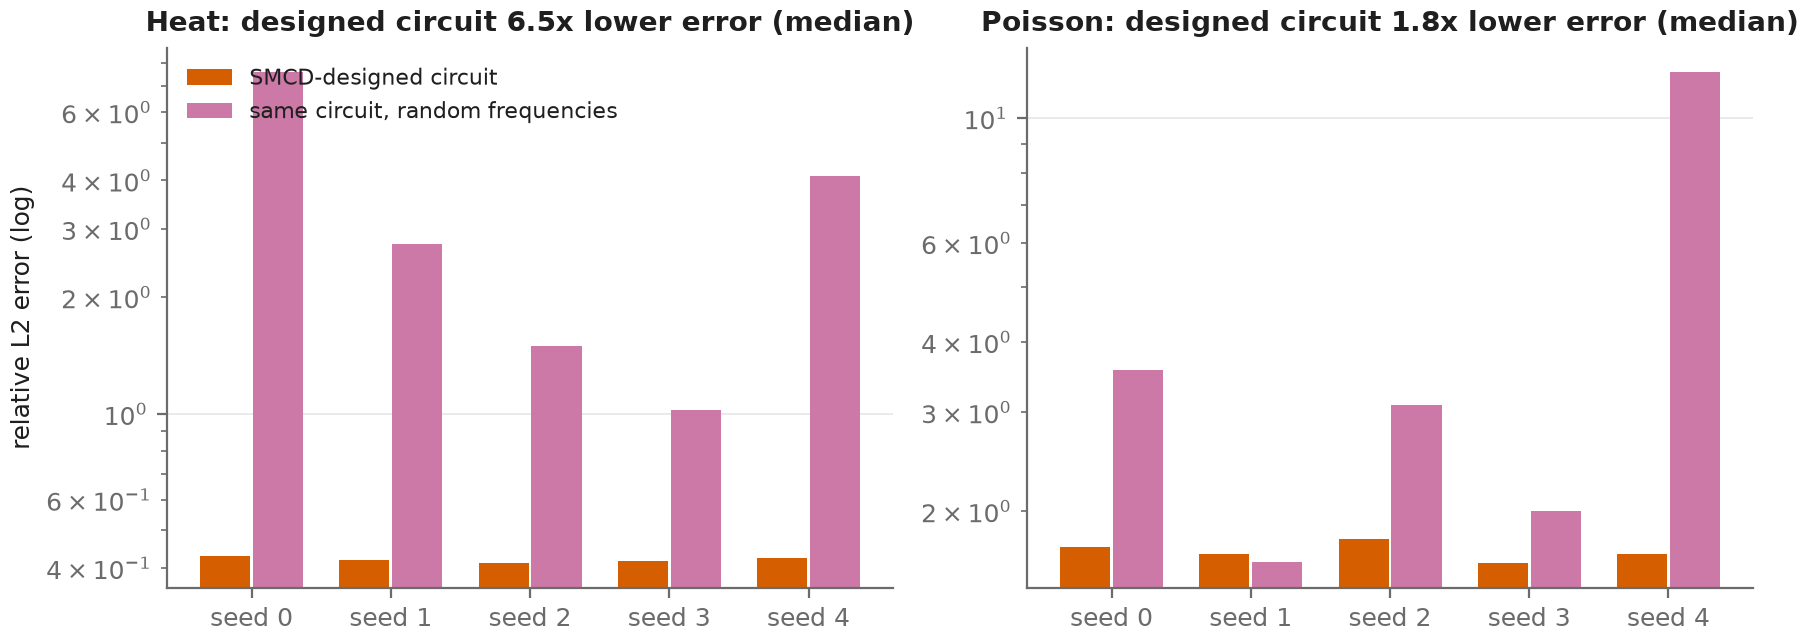
\includegraphics[width=\linewidth]{../results/report/figures/headline_design_vs_random.png}
  \caption{One copy of the circuit with SMCD's scalings against the same circuit with
    random scalings, every seed, heat (left) and Poisson (right).}
  \label{fig:designrandom}
\end{figure}

\subsection{The mechanism in the frequency domain}
\label{sec:mechanism}

\paragraph{The gain lands on the designed frequencies.} Projecting the error onto Fourier
modes and accumulating the improvement over the MLP frequency by frequency, 99.9\% of the
circuit's improvement on Poisson lies inside $\Omega$ with one copy, 99.9\% with eight,
and 99.4\% on groundwater (the bar was 70\%). On Helmholtz $k{=}10$ the circuit improves
on the MLP at no frequency at all, so there is nothing to attribute
(Figure~\ref{fig:heatmaps}).

\paragraph{The NTK is flatter inside $\Omega$ once the model can express it.} Proposition~4
predicts a flatter NTK spectrum inside the encoded band. With eight copies on Poisson the
decay exponent inside $\Omega$ is flatter than outside by 15.2 (the bar was 0.5). With one
copy the comparison cannot be made on Poisson: the model has 14 parameters, so its NTK has
at most 14 non-zero eigenvalues and none beyond index $|\Omega|=81$. On Helmholtz
$k{=}10$, where every model fails, the spectrum is steeper inside $\Omega$ (gap $-8.4$)
(Figure~\ref{fig:ntk}).

\paragraph{Hybrid models stay closer to their initial kernel.} The prediction that
hybrids leave the lazy-training regime earlier is reversed: at 5{,}000 steps the median
relative NTK drift is 1.0 for the one-copy hybrid and $4.3\times10^6$ for the classical
models (2.5 against $9.7\times10^4$ with eight copies). The circuits also use few
directions in parameter space: an NTK effective rank of 1.4 on Poisson and 1.1 on heat,
and a Fisher effective dimension of about 4, flat through training, where the MLP's grows
from about 4 to 12 (Poisson) and 5 to 50 (heat). The size-matched classical model looks
like the circuit (effective rank 2.0 and 1.9), so this is mostly an effect of size, not of
being quantum (Figure~\ref{fig:evolution}).

\paragraph{Coverage alone does not predict error.} SMCD's design card reports the
fraction of the target spectrum inside $\Omega$. Sweeping the coverage target on Poisson
builds only three distinct circuits (a target of 0.8, 0.9 or 1.0 yields the same one), so
coverage there is confounded with parameter count, and at the full training budget the
correlation between coverage and error is $\rho=+0.29$, the wrong sign for the
pre-registered $\rho\le-0.7$. On Helmholtz $k{=}10$ every target builds the same circuit,
which scores about 1 throughout. Covering the band is necessary for the design to help
(Section~\ref{sec:design}) but not sufficient for a single circuit to train well.

\paragraph{No measurable barren plateau at this scale.} Gradient variance fitted against
qubit count (4 and 6 qubits, three seeds) has slope 0.31, under the $\log2=0.69$ bar, but
the fit explains almost none of the variation ($R^2=0.001$): no decay is detectable
between 4 and 6 qubits. Eight qubits did not fit in the simulator's memory.

\begin{figure}[htbp]
  \centering
  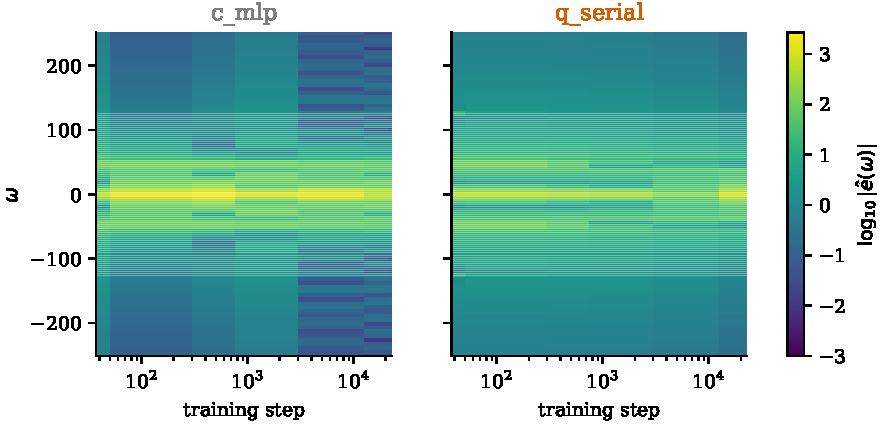
\includegraphics[width=\linewidth]{figures/freq_heatmap_poisson.pdf}\\[4pt]
  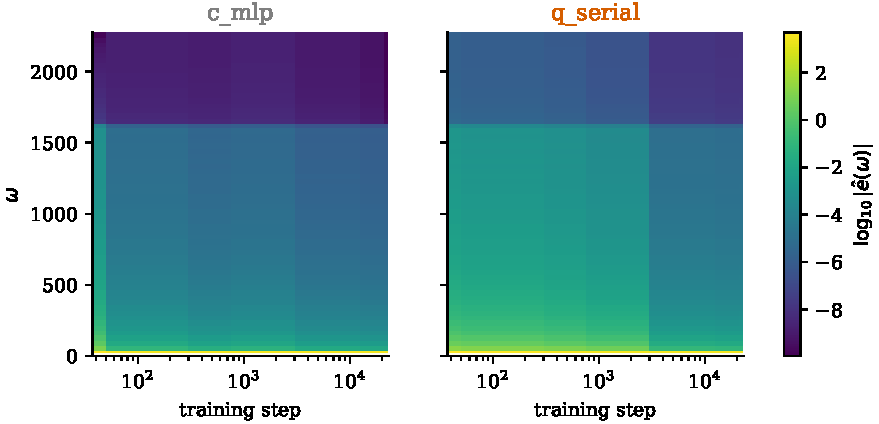
\includegraphics[width=\linewidth]{figures/freq_heatmap_helmholtz_k10.pdf}
  \caption{Per-frequency error $|\hat e(\omega)|$ over training, MLP (left,
    \texttt{c\_mlp}) against one copy of the SMCD circuit (right, \texttt{q\_serial}),
    seed 0, with $\Omega$ overlaid as thin white lines.
    Top: Poisson, two-sided spectrum within $\pm2\max|\Omega|$. Bottom: Helmholtz
    $k{=}10$, radially binned; all of $\Omega$ ($|\omega|\le19$) falls in the lowest bin.}
  \label{fig:heatmaps}
\end{figure}

\begin{figure}[htbp]
  \centering
  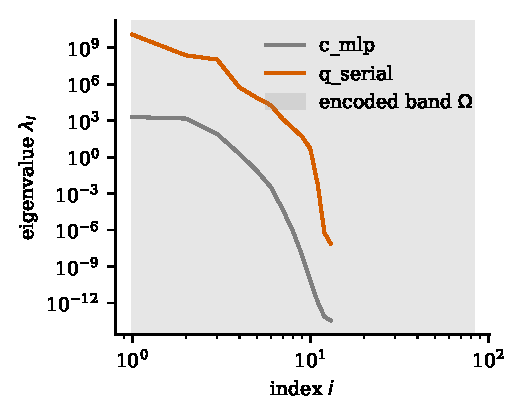
\includegraphics[width=0.48\linewidth]{figures/ntk_spectrum_poisson_pr7.pdf}\hfill
  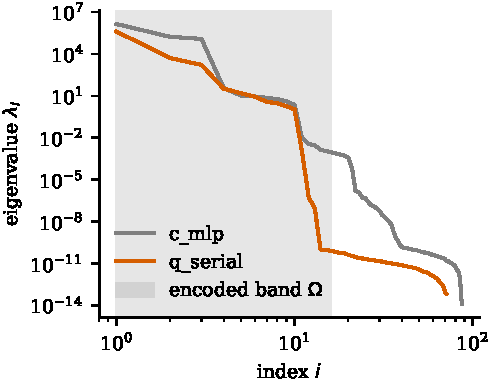
\includegraphics[width=0.48\linewidth]{figures/ntk_spectrum_helmholtz_k10_pr7.pdf}
  \caption{Residual NTK eigenvalue spectra at the final checkpoint, MLP
    (\texttt{c\_mlp}) against one copy of the SMCD circuit (\texttt{q\_serial}), seed 0,
    with the top-$|\Omega|$ index range shaded. Left:
    Poisson ($|\Omega|=81$ exceeds the circuit's 14 parameters). Right: Helmholtz
    $k{=}10$ ($|\Omega|=15$).}
  \label{fig:ntk}
\end{figure}

\subsection{Why one copy is not enough}
\label{sec:copyresult}

\paragraph{One copy learns the hard frequency and loses the easy one.} The Poisson
solution is $\sin\pi x+0.3\sin15\pi x$. Tracking the error at those two frequencies
(Figure~\ref{fig:specerr}), one copy cuts its $15\pi$ error to a median 10\% of its
starting value by step 1{,}000 (103\% for the Fourier-feature network, 86\% for the MLP,
51\% for the frequency-matched model). Its $\pi$ error falls to about 30\% by step
5{,}000 and then \emph{rises} to 1.9--2.0$\times$ its starting value by step 20{,}000, on
all five seeds, while the frequency-matched model reduces both. The residual loss weights
each Fourier mode of the error by $\omega^2$, so the $15\pi$ mode carries 225 times the
weight of the $\pi$ mode. A linear head on fixed sine features sets the two amplitudes
independently; a single circuit cannot, because all 81 of its amplitudes are functions of
the same ten angles read through one expectation value. Our reading, supported by these
data but not proven, is that the optimiser buys the heavily weighted amplitude at the
cost of the lightly weighted one. The loss agrees: it stalls near $3.3\times10^4$ from
step 1{,}000 while the error keeps moving, and the seeds agree closely (worst over best
$1.1\times$) because they converge to the same trade-off.

\begin{figure}[htbp]
  \centering
  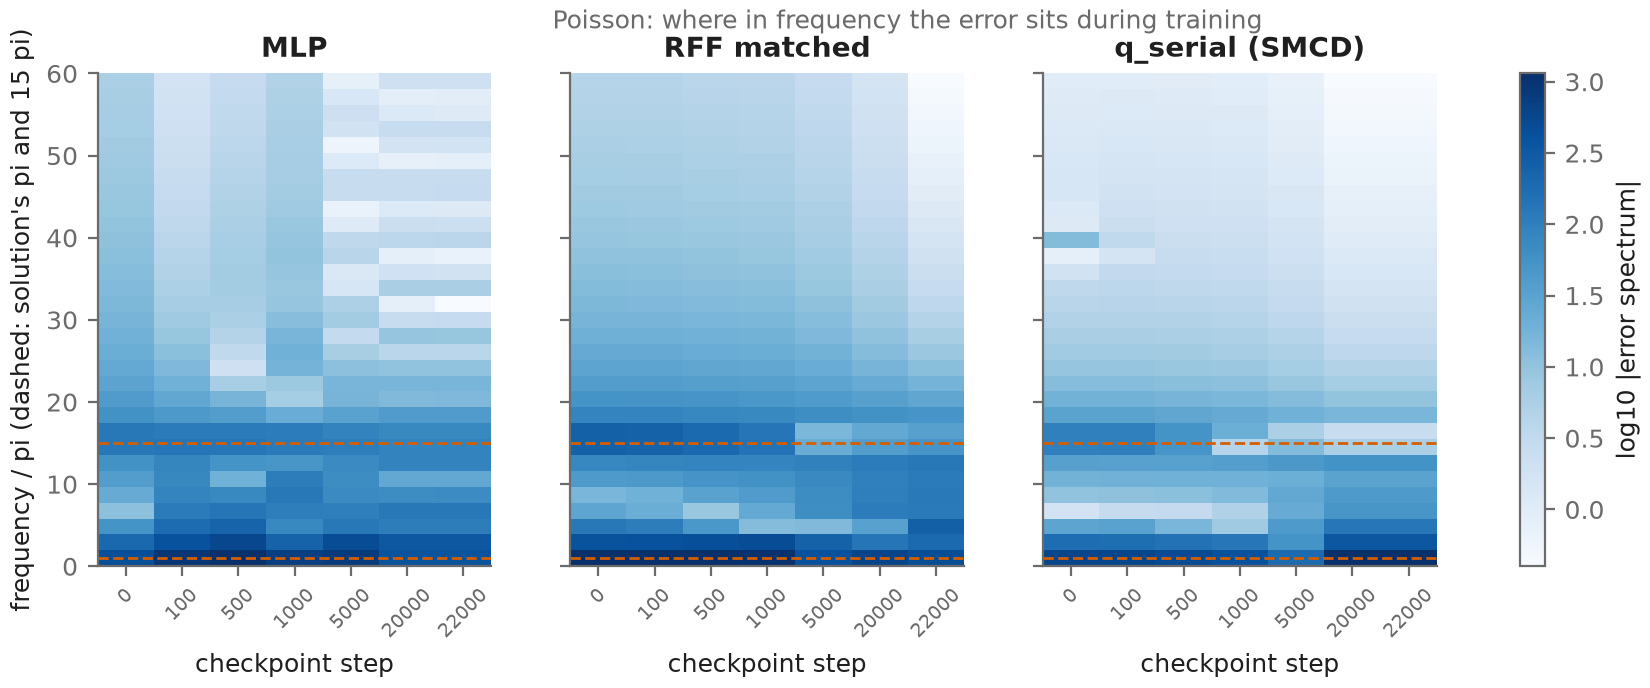
\includegraphics[width=\linewidth]{../results/report/figures/xai_spectral_error_poisson.png}
  \caption{Poisson, one copy: magnitude of the error spectrum at each checkpoint
    (seed 0), with the error at $\pi$ and $15\pi$ tracked over training.}
  \label{fig:specerr}
\end{figure}

\paragraph{Copies decouple the amplitudes.} Section~\ref{sec:copies}'s copies keep
$\Omega$ and give the head an independent handle on each copy. On the tuning seeds the
error falls with the number of copies, from 1.67 with one copy to 0.003 with eight at the
higher learning rate (Figure~\ref{fig:copies}); eight copies were selected.

\begin{figure}[htbp]
  \centering
  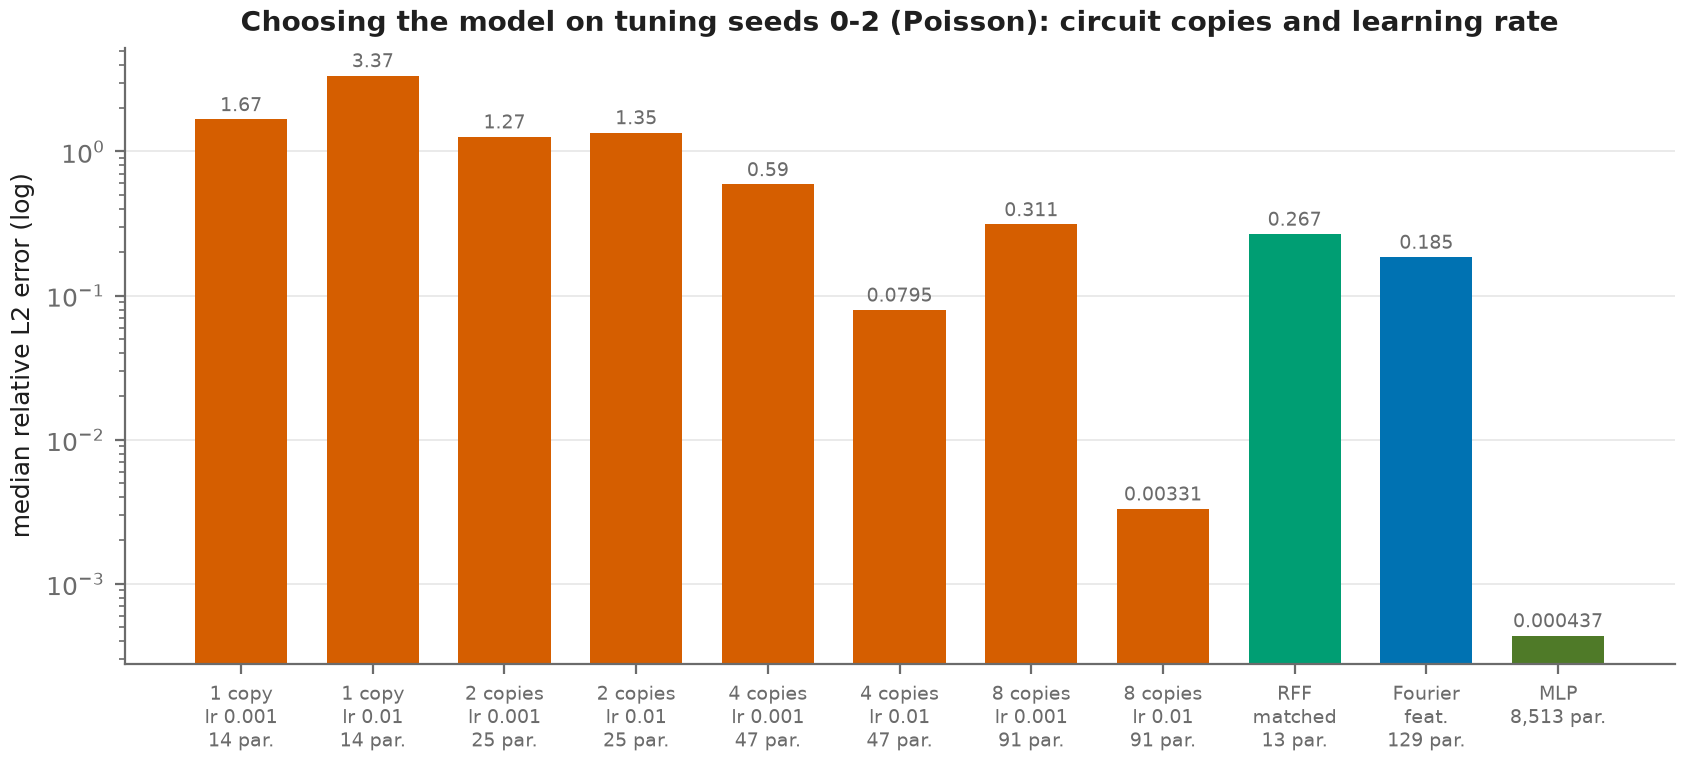
\includegraphics[width=\linewidth]{../results/report/figures/headline_v2_lab.png}
  \caption{Model selection on Poisson, tuning seeds 0--2: median error for 1, 2, 4 and 8
    copies at two learning rates, beside the best learning rate for each classical model.}
  \label{fig:copies}
\end{figure}

\paragraph{Eight copies on held-out seeds.} On seeds 10--14 (Table~\ref{tab:ensemble},
Figure~\ref{fig:ensemble}) the eight-copy circuit reaches a median error of 0.0037, with
every seed below 0.02. It beats the Fourier-feature network by three orders of magnitude
and the same circuit with random frequencies by $236\times$. The comparison with the MLP is
inconclusive: at its tuned learning rate the MLP failed on three of five seeds (1.2--3.6)
and reached 0.003--0.012 on the other two. The classical learning rates chosen on the
tuning seeds did not transfer well (the Fourier-feature network went from 0.19 to 5.0),
which inflates both of those ratios. \textbf{The frequency-matched classical model,
sized to the eight-copy circuit (83 parameters), is $3.3\times$ more accurate} (0.0011):
on Poisson, handing a classical model the frequencies SMCD reads off the equation works
better than the circuit.

% Generated by scripts/report/paper_tables.py from results/adjudication_v2.json.
\begin{table}[htbp]
  \centering
  \small
  \begin{tabular}{p{0.5\linewidth}lr}
  \toprule
  Claim & Verdict & Measured \\
  \midrule
  Beats the large MLP on Poisson ($\ge2\times$) & Inconclusive & 337.79$\times$ \\
  Beats Fourier features on Poisson ($\ge1.3\times$) & \textbf{Confirmed} & 1359.81$\times$ \\
  Matches the frequency-matched classical model on Poisson (within $1.3\times$) & Refuted & 3.30$\times$ \\
  Designed beats random frequencies, Poisson ($\ge1.5\times$) & \textbf{Confirmed} & 236.08$\times$ \\
  NTK flatter inside $\Omega$ than outside, Poisson & \textbf{Confirmed} & gap 15.2 \\
  Gain over the MLP lies inside $\Omega$, Poisson ($\ge70\%$) & \textbf{Confirmed} & 99.9\% \\
  Leaves the lazy-training regime earlier than classical models & Refuted & 2.53 vs 9.7e+04 \\
  Encoder drift stays below 0.2, so $\Omega$ stays valid & \textbf{Confirmed} & 0.10 \\
  \midrule
  Confirmed & 5 of 8 & \\
  \bottomrule
  \end{tabular}
  \caption{Pre-registered claims about the eight-copy SMCD circuit on Poisson, held-out seeds
    10--14. The baselines are sized to the eight-copy circuit where the claim names one.}
  \label{tab:ensemble}
\end{table}


\begin{figure}[htbp]
  \centering
  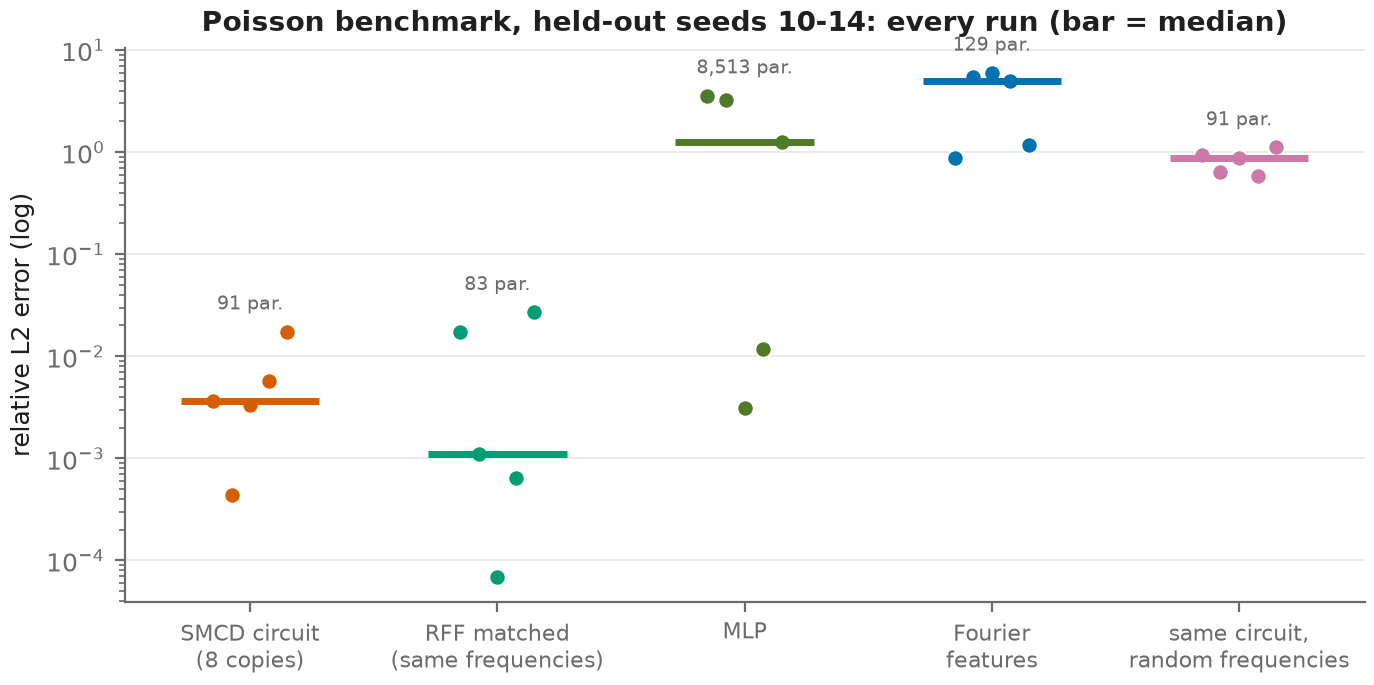
\includegraphics[width=0.9\linewidth]{../results/report/figures/headline_v2_retest.png}
  \caption{Poisson, held-out seeds 10--14: every run of the eight-copy circuit and the
    baselines (bar: median).}
  \label{fig:ensemble}
\end{figure}
